\section{Experiments}
\label{sec:experiments}

\vspace{-2mm}

We extensively evaluate \implname on multiple tasks and models with the purpose of:
(1) assessing the efficiency and effectiveness of \svdacro;
(2) demonstrating self-adaptiveness through the three proposed adaptation strategies;
(3) conducting in-depth analysis and ablation studies aimed at understanding and interpreting the properties of our new framework.

\vspace{-2mm}
\subsection{Experimental setups}
\vspace{-1mm}

To validate the generality of \implname we consider three pre-trained LLMs ranging across different model families and architecture sizes: \llama, \mistral, and \llamaXL.
For each model, we obtain three sets of \svdacro-trained $z$ vectors to maximize performance for GSM8K~\citep{cobbe2021training},  MBPP-pro~\citep{austin2021program}, and ARC-Easy~\citep{clark2018think}, respectively.
Additionally, we also train a set of $z$ vectors for \llama, when applied as the language backbone for TextVQA~\citep{singh2019towards}, in order to assess \svdacro's applicability to the vision-language modeling (VLM) domain.
We provide \svdacro's main learning curves on each of these tasks in Figure~\ref{fig:learning_curves}. 
Finally, we evaluate the full \implname adaptation framework on four unseen tasks: MATH~\citep{hendrycks2021measuring}, Humaneval~\citep{chen2021evaluating}, ARC-Challenge~\citep{clark2018think}, and OKVQA~\citep{marino2019ok}. In all our adaptation experiments, we only consider experts obtained in the pure-language settings, assessing its test-time applicability even for the distinctive vision domain. 
Please refer to the Appendix~\ref{app:sec:implementation} for additional details and a summary of the hyper-parameters used in the experiments.

\begin{figure}[!t]
    \centering
    % \vspace{-4mm}
    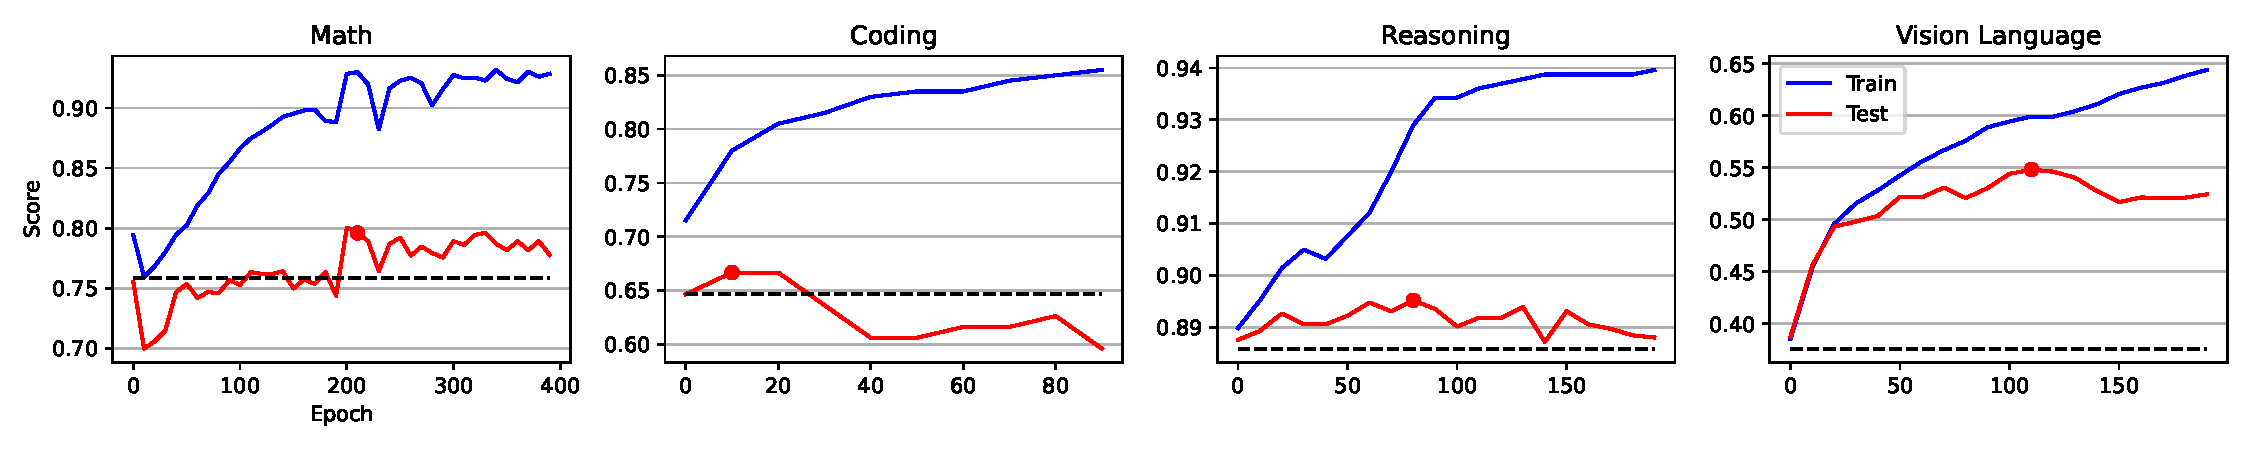
\includegraphics[width=0.95\textwidth]{images/learning_curves_new.pdf}
    \vspace{-4mm}
    \caption{\textbf{\svdacro learning curves.} The dashed lines indicate the performance of \llama on the test split of each task. SVF effectively fine-tunes to surpass the base performance. While we use the best validation score to select our checkpoint for evaluation (marked by red dots), we present the entire training curve without early stopping to demonstrate \svdacro's learning capabilities. Tasks with only hundreds of training samples like Coding and Reasoning were stopped early. In our experiments, we update the parameters at the end of each epoch.}
    \vspace{-6mm}
    \label{fig:learning_curves}
\end{figure}


\subsection{Experimental results}

% \begin{table}[!t]
% \centering

% \caption{\textbf{LLM Fine-tuning Results.} LLM performance on the test splits.}

% \small
% \begin{tabular}{llll}
% \toprule

% \textbf{Method} & \textbf{GSM8K} & \textbf{MBPP-Pro} & \textbf{ARC-Easy} \\

% \midrule
% \llama & {\normalsize 75.89 {\footnotesize (\grey{1.00})}} & {\normalsize 64.65 {\footnotesize (\grey{1.00})}} & {\normalsize 88.59 {\footnotesize (\grey{1.00})}} \\
% \quad + LoRA & {\normalsize 70.58 {\footnotesize (\red{0.93})}} & \textbf{{\normalsize 67.68 {\footnotesize (\green{1.05})}}} & {\normalsize 88.97 {\footnotesize (\grey{1.00})}} \\
% \quad + SVF (Ours) & \textbf{{\normalsize 79.15 {\footnotesize (\green{1.04})}}} & {\normalsize 66.67 {\footnotesize (\green{1.03})}} & \textbf{{\normalsize 89.56 {\footnotesize (\green{1.01})}}} \\

% \midrule
% \mistral & {\normalsize 42.83 {\footnotesize (\grey{1.00})}} & {\normalsize 49.50 {\footnotesize (\grey{1.00})}} & {\normalsize 49.50 {\footnotesize (\grey{1.00})}} \\
% \quad + LoRA & {\normalsize 36.09 {\footnotesize (\red{0.84})}} & {\normalsize 47.47 {\footnotesize (\red{0.96})}} & {\normalsize 47.47 {\footnotesize (\red{0.96})}} \\
% \quad + SVF (Ours) & \textbf{{\normalsize 49.74 {\footnotesize (\green{1.16})}}} & \textbf{{\normalsize 51.52 {\footnotesize (\green{1.04})}}} & \textbf{{\normalsize 85.14 {\footnotesize (\green{1.72})}}} \\

% \midrule
% \llamaXL & {\normalsize 85.29 {\footnotesize (\grey{1.00})}} & \textbf{{\normalsize 80.81 {\footnotesize (\grey{1.00})}}} & \textbf{{\normalsize 89.10 {\footnotesize (\grey{1.00})}}} \\
% \quad + SVF (Ours) & \textbf{{\normalsize 88.32 {\footnotesize (\green{1.04})}}} & \textbf{{\normalsize 80.81 {\footnotesize (\grey{1.00})}}} & {\normalsize 88.47 {\footnotesize (\red{0.99})}} \\

% \bottomrule
% \end{tabular}

% \label{tab:res:svf_train_tasks}
% \end{table}

% \begin{figure}[!t]
%     \centering
%     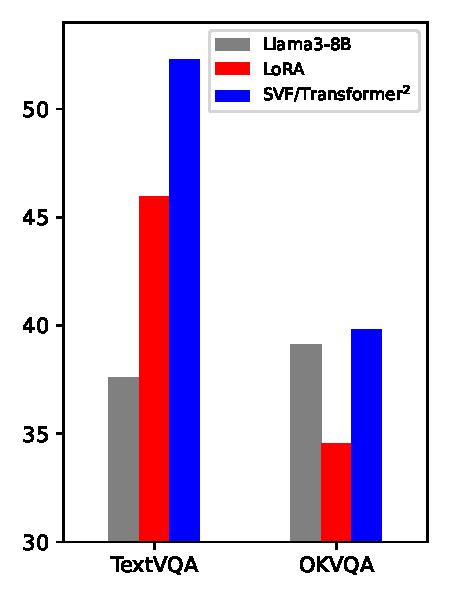
\includegraphics[width=\textwidth]{images/vlm_barplot.pdf}
%     % \vspace{-8mm}
%     \caption{\textbf{VLM Results.}
%     }
%     % \vspace{-4mm}
%     \label{fig:vlm_results}
% \end{figure}



\begin{figure}[!b]
    \vspace{-4mm}
    \centering

    % Left side: Table
    \begin{minipage}{0.75\linewidth}
        \centering
        \captionof{table}{\textbf{Fine-tuning results.} LLM performance on the test splits of math, coding and reasoning. Normalized scores are in the parentheses.}
        \vspace{-3.5mm}
        \small
        \begin{tabular}{llll}
            \toprule
            \textbf{Method} & \textbf{GSM8K} & \textbf{MBPP-Pro} & \textbf{ARC-Easy} \\
            \midrule
            \llama & {\normalsize 75.89 {\scriptsize (\grey{1.00})}} & {\normalsize 64.65 {\scriptsize (\grey{1.00})}} & {\normalsize 88.59 {\scriptsize (\grey{1.00})}} \\
            \quad + LoRA & {\normalsize 77.18 {\scriptsize (\green{1.02})}} & \textbf{{\normalsize 67.68 {\scriptsize (\green{1.05})}}} & {\normalsize 88.97 {\scriptsize (\grey{1.00})}} \\
            \quad + SVF (Ours) & \textbf{{\normalsize 79.15 {\scriptsize (\green{1.04})}}} & {\normalsize 66.67 {\scriptsize (\green{1.03})}} & \textbf{{\normalsize 89.56 {\scriptsize (\green{1.01})}}} \\
            \midrule
            \mistral & {\normalsize 42.83 {\scriptsize (\grey{1.00})}} & {\normalsize 49.50 {\scriptsize (\grey{1.00})}} & {\normalsize 81.65 {\scriptsize (\grey{1.00})}} \\
            \quad + LoRA & {\normalsize 44.66 {\scriptsize (\red{1.04})}} & {\normalsize 51.52 {\scriptsize (\green{1.04})}} & {\normalsize 81.19 {\scriptsize (\red{0.98})}} \\
            \quad + SVF (Ours) & \textbf{{\normalsize 49.74 {\scriptsize (\green{1.16})}}} & \textbf{{\normalsize 51.52 {\scriptsize (\green{1.04})}}} & \textbf{{\normalsize 85.14 {\scriptsize (\green{1.04})}}} \\
            \midrule            
            \llamaXL & {\normalsize 85.29 {\footnotesize (\grey{1.00})}} & \textbf{{\normalsize 80.81 {\footnotesize (\grey{1.00})}}} & \textbf{{\normalsize 89.10 {\footnotesize (\grey{1.00})}}} \\
            \quad + LoRA & {\normalsize 77.26 {\footnotesize (\red{0.91})}} & {\normalsize 68.69 {\footnotesize (\red{0.85})}} & {\normalsize 88.55 {\footnotesize (\red{0.99})}} \\
            \quad + SVF (Ours) & \textbf{{\normalsize 88.32 {\footnotesize (\green{1.04})}}} & \textbf{{\normalsize 80.81 {\footnotesize (\grey{1.00})}}} & {\normalsize 88.47 {\footnotesize (\red{0.99})}} \\
            \bottomrule                
        \end{tabular}
        \label{tab:res:svf_train_tasks}
    \end{minipage}
    \hfill
    % Right side: Figure
    \begin{minipage}{0.23\linewidth}
        \centering
        % \vspace{2mm}
        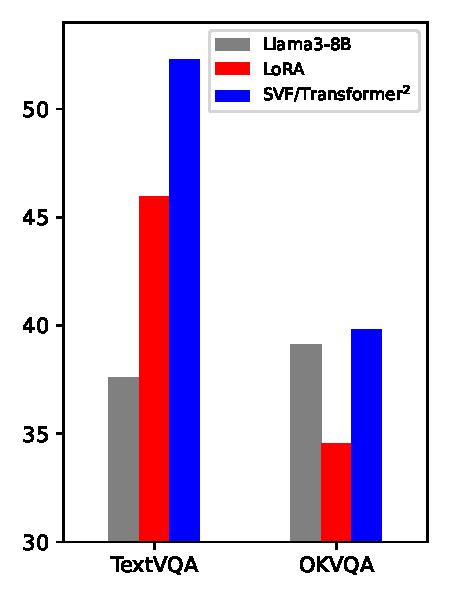
\includegraphics[width=\linewidth]{images/vlm_barplot.pdf}
        \vspace{-8mm}
        \captionof{figure}{\textbf{Results for the VLM domain.}}
        \label{fig:vlm_results}
    \end{minipage}

\end{figure}


\textbf{\svdacro performance}
We provide results after training on each considered task with the \llama, \mistral, and \llamaXL base models in Table~\ref{tab:res:svf_train_tasks}.
Remarkably, we find that \svdacro provides considerable and consistent performance gains across nearly all tasks and base models. Instead, LoRA experts yield smaller gains and even sporadic performance degradation.
(These LoRA experts are trained with next token prediction. While we also have LoRA experts trained with RL in Table~\ref{tab:res:ablation}, RL seems work less well with LoRA than with \svdacro.)
This observed trend extends also to the vision-language domain, as fine-tuning \textsc{Llama3-Llava-Next-8B} with \svdacro bolsters the base model's performance by over 39\% (see Figure~\ref{fig:vlm_results}).
To ensure a fair comparison, we provide extensive ablations to both our model and the LoRA baseline considering different architecture and optimization objectives in Appendix~ \ref{app:sec:ablation_studies}).
Due to its essential parameterization, we would like to note that training \svdacro requires considerably fewer resources, with less than 10\% of the training parameters of our LoRA implementation.

\textbf{Adaptation performance}
With the \svdacro trained $z$ vectors, we assess the self-adaptation capability of \implname on unseen tasks.
For a fair comparison with LoRA, we record the performance of this baseline using all checkpoints from the considered training tasks and report only its highest performance for each of the test tasks. 
As shown in Table~\ref{tab:res:svf_ada_tasks}, all of our \implname adaptation strategies demonstrate improvements across all tasks for \llama base models, and in at least two out of three tasks for both \mistral and \llamaXL.
In contrast, even the best training LoRAs only provide marginal improvements on the ARC-Challenge task and still significantly deteriorate performance on both MATH and Humaneval. 
This discrepancy suggests that LoRA's parameterization and optimization might be particularly sensitive to overfitting, especially when trained with the smaller GSM8K and MBPP-Pro datasets, the tasks that provide information most related to MATH and Humaneval.
In Figure~\ref{fig:vlm_results}, we find a similar dichotomy in the OKVQA task, with the performance of the base \textsc{Llama3-Llava-Next-8B} VLM only improving after applying \implname.
We note that also in this setting, \implname performs self-adaptation only from the expert vectors from GSM8K, MBPP-Pro, and ARC-Easy.
Thus, this result further underscores the high flexibility of self-adaptation, transferring knowledge compressed for tasks entirely based on language even for unrelated vision-based problems.

\begin{table}[!t]
\centering
\vspace{-2mm}
\caption{\textbf{Self-adaptation on unseen tasks.} Normalized scores are in the parentheses.}
% \vspace{-2mm}
\small
\begin{tabular}{llll}
\toprule
Method & MATH & Humaneval & ARC-Challenge \\

\midrule
\llama3 & {\normalsize 24.54 {\footnotesize (\grey{1.00})}} & {\normalsize 60.98 {\footnotesize (\grey{1.00})}} & {\normalsize 80.63 {\footnotesize (\grey{1.00})}} \\
\quad + LoRA & {\normalsize 21.68 {\footnotesize (\red{0.88})}} & {\normalsize 52.44 {\footnotesize (\red{0.86})}} & {\normalsize 81.06 {\footnotesize (\green{1.01})}} \\
\quad + \implname (Prompt) & {\normalsize 25.22 {\footnotesize (\green{1.03})}} & {\normalsize 61.59 {\footnotesize (\green{1.01})}} & {\normalsize 81.74 {\footnotesize (\green{1.01})}} \\
\quad + \implname (Cls-expert) & {\normalsize 25.18 {\footnotesize (\green{1.03})}} & {\normalsize 62.80 {\footnotesize (\green{1.03})}} & {\normalsize 81.37 {\footnotesize (\green{1.01})}} \\
\quad + \implname (Few-shot) & \textbf{{\normalsize 25.47 {\footnotesize (\green{1.04})}}} & \textbf{{\normalsize 62.99 {\footnotesize (\green{1.03})}}} & \textbf{{\normalsize 82.61 {\footnotesize (\green{1.02})}}} \\

\midrule
\mistral & {\normalsize 13.02 {\footnotesize (\grey{1.00})}} & {\normalsize 43.29 {\footnotesize (\grey{1.00})}} & {\normalsize 71.76 {\footnotesize (\grey{1.00})}} \\
\quad + LoRA & {\normalsize 11.18 {\footnotesize (\red{0.86})}} & {\normalsize 31.71 {\footnotesize (\red{0.73})}} & \textbf{{\normalsize 75.77 {\footnotesize (\green{1.06})}}} \\
\quad + \implname (Prompt) & {\normalsize 11.86 {\footnotesize (\red{0.91})}} & {\normalsize 43.90 {\footnotesize (\green{1.01})}} & {\normalsize 72.35 {\footnotesize (\green{1.01})}} \\
\quad + \implname (Cls-expert) & {\normalsize 11.60 {\footnotesize (\red{0.89})}} & {\normalsize 43.90 {\footnotesize (\green{1.01})}} & {\normalsize 74.83 {\footnotesize (\green{1.04})}} \\
\quad + \implname (Few-shot) & \textbf{{\normalsize 13.39 {\footnotesize (\green{1.03})}}} & \textbf{{\normalsize 47.40 {\footnotesize (\green{1.09})}}} & {\normalsize 75.47 {\footnotesize (\green{1.05})}} \\

\midrule
\llamaXL & \textbf{{\normalsize 40.64 {\footnotesize (\grey{1.00})}}} & {\normalsize 78.66 {\footnotesize (\grey{1.00})}} & {\normalsize 87.63 {\footnotesize (\grey{1.00})}} \\
\quad + LoRA & {\normalsize 25.40 {\footnotesize (\red{0.62})}} & {\normalsize 73.78 {\footnotesize (\red{0.94})}} & {\normalsize 83.70 {\footnotesize (\red{0.96})}} \\
\quad + \implname (Prompt) & {\normalsize 40.44 {\footnotesize (\grey{1.00})}} & \textbf{{\normalsize 79.88 {\footnotesize (\green{1.02})}}} & \textbf{{\normalsize 88.48 {\footnotesize (\green{1.01})}}} \\
\bottomrule

\end{tabular}

\label{tab:res:svf_ada_tasks}
\vspace{-6mm}
\end{table}



Comparing the three proposed adaptation strategies, we highlight a clear monotonic trend -- with more involved strategies and additional information about the test-time condition, self-adaptation appears to be increasingly effective.
In particular, \implname with few-shot self-adaptation is almost always the highest-scoring method, providing notable improvements across all tested settings except for \llamaXL@MATH, where we have only SVF-tuned half of the layers due to our limited GPU resources.
This trend shows that providing additional or different kinds of information seems to be highly beneficial to our framework, suggesting that \implname could provide foundation models with new means to continually improve performance when deployed in lifelong settings.

\begin{wraptable}{r}{0.35\textwidth}
\vspace{-6mm}
\centering
\caption{\textbf{Time cost of 2-pass inference in prompt adaptation strategy of \implname for the entire problem set.} 1st to 2nd pass inference time ratios are shown in parentheses.}
\label{tab:res:inference_time}
\vspace{-3.5mm}
\small
\resizebox{0.35\textwidth}{!}{
\begin{tabular}{lrr}
\toprule
\textbf{Task} & \textbf{1st (s)} & \textbf{2nd (s)} \\
\midrule
MATH         & 42.64    {\footnotesize (13\%)}             & 321.19                  \\
Humaneval    & 2.76   {\footnotesize (19\%)}                 & 14.28                   \\
ARC-Challenge & 13.40      {\footnotesize (47\%)}             & 28.51                   \\
\bottomrule
\end{tabular}
}
\vspace{-4mm}
\end{wraptable}

Table~\ref{tab:res:inference_time} reports the inference time required by the prompt adaptation strategy of \implname, with the time spent on solving the entire problem set presented separately for the 1st and 2nd passes.
Notice that the 2nd pass inference time is the time spent on solving the problems, and the 1st pass inference time is the time for self-adaptation, 1st to 2nd pass inference time ratios are in the parentheses.
While the additional inference pass might appear to double the overall runtime, it is important to note that inference time primarily depends on the number of tokens generated.
In our settings, it is $\mathcal{O}(n)$ where $n$ is the length of the input.
ARC-challenge's cost ratio is large because they are single choice problems and therefore the cost of the 2nd pass is also $\mathcal{O}(n)$.
In general settings, we think it is reasonable to assume this ratio to be closer to those of MATH and Humaneval.
For a detailed discussion on improving the efficiency of CEM few-shot adaptation methods, please see Appendix~\ref{app:sec:efficiency_improvements}

\subsection{Analysis}
\label{sec:analysis}

Lastly, we analyze and discuss the properties of our adaptation strategies for which we provide extensions and further discussion Appendix~\ref{app:sec:additional_exp}.

\textbf{Analysis 1: Job dispatching accuracy}
In Figure~\ref{fig:confusion_matrices} we provide the confusion matrices of our classification-based adaptation strategies. These results validate the effectiveness of both our classification-based adaptation strategies to match each prompt with experts trained in similar domains, as evidenced by the high values along the diagonals. 
Furthermore, the results from \llama and \mistral also show that using the classification expert consistently provides higher classification accuracy than vanilla prompt engineering.
While this difference could explain the higher performance of the relative self-adaptation strategy, we also note that domain similarity might not be the only metric relevant to identifying the best expert for each prompt or task.
To this end, we believe many further unexplored extensions could be explored in future work, using heuristics such as past expert performance or token-level analysis to further push our framework's scalability.

\begin{figure}[t]%[!b]
    \centering
    \vspace{-0.5mm}
    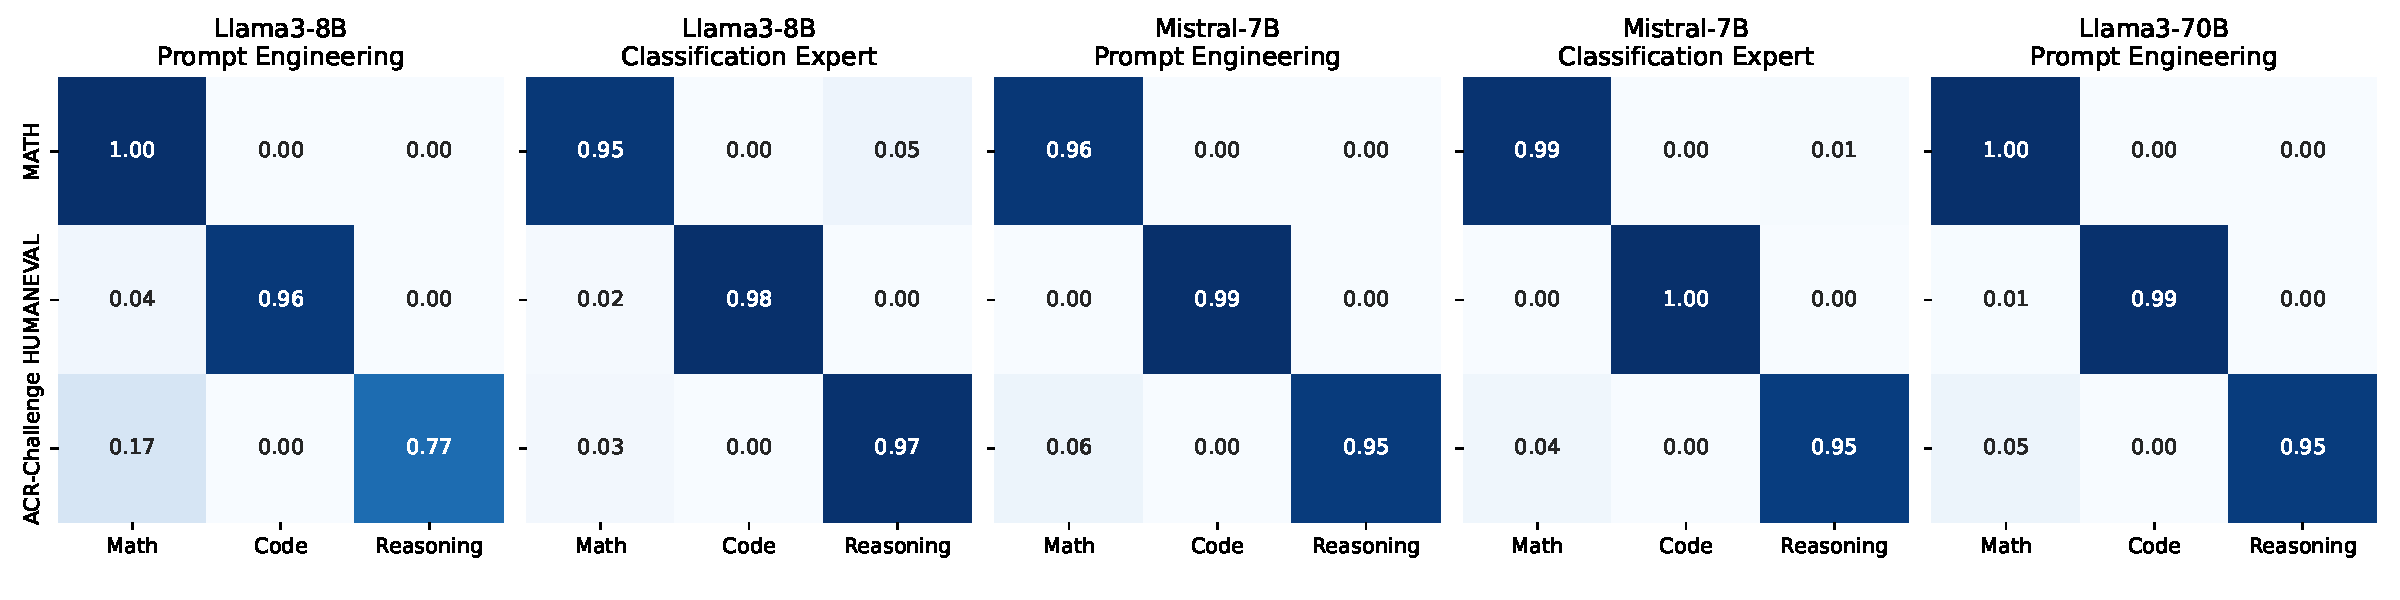
\includegraphics[width=0.9\textwidth]{images/confusion_matrices.pdf}
    \vspace{-4mm}
    \caption{\textbf{Confusion matrices.} These matrices display the classification percentages, where rows represent the task classes (ground truth) and columns indicate the predicted categories. Some samples are misclassified as ``Others,'' which is reflected in rows where the totals do not sum to one.
    }
    \vspace{-10mm}
    \label{fig:confusion_matrices}
\end{figure}

\textbf{Analysis 2: Training tasks adaptation contribution}
In Figure~\ref{fig:cem}, we show the normalized adaptive coefficients $a_k$ interpolating between our \svdacro vectors learned via CEM for \llama and \mistral across all the unseen downstream tasks. 
Intuitively, we find that the expert vectors from the training tasks sharing similar topics to the unseen ones are often the highest contributors to the produced adaptive weights. 
However, we observe that the MATH task appears as an interesting exception, as the $a_k$ for the expert obtained from GSM8K training is actually the lowest out of the three in both models.
We hypothesize this reflects the different nature of the mathematics competition problems from MATH as compared to the grade-school problems in GSM8K.
In fact, not only is the difficulty of the MATH questions far beyond GSM8K, but a large portion of its problems also hinges mainly on logical reasoning, for which a task like ARC might actually be more aligned.
Furthermore, we also note that the different $z$ vectors appear to contribute more uniformly to adaptation in the Llama model.
This difference might indicate that, due to its higher base performance, the Llama model does not need to rely on any particular set of skills as much as Mistral, and can harness more holistic benefits from self-adaptation.
Note that applying $a_k$ uniformly is not a universal solution for leveraging expert vectors. This becomes evident when we look at different model and task combinations (e.g. applying $a_k$ uniformly on \llama for MATH tasks only achieves 24.47, while \implname(Few-shot) achieves 25.47).

\textbf{Analysis 3: Ablation studies}

\label{app:sec:ablation_studies}

\textit{Module sensitivity:} We first compare the performance of \svdacro when it is applied to different modules (see trials 1-3).
Under consistent conditions, both individual MLP and attention updates improve performance, with MLP updates resulting in more pronounced gains.
Simultaneous updates to both module types yield even more significant enhancements.

\textit{Objective function:} We are interested in the performance impact from different objective functions, and we compare the RL objective with next-token prediction loss (see trials 2 and 4).
For the latter, we use instruction fine-tuning with official GSM8K solutions as target tokens.
Results show clear performance gains with RL, demonstrating its effectiveness in task-specific fine-tuning.
Conversely, next-token prediction even hinders performance.
This highlights RL's ability to handle cases lacking detailed solutions, suggesting its superiority in this context.

\textit{\svdacro vs LoRA:} Finally, we also evaluate LoRA using the RL objective (see trials 2 and 5).
A significant performance disparity is observed, primarily attributed to the severe instability of the LoRA training process.
Despite exploring a wide range of learning rates, LoRA's performance consistently lagged behind.
For further illustrations, see Figure~\ref{app:fig:lora_learning_curves} in the appendix.
\begin{table}[h]
% \begin{table}[!b]

% \vspace{-2mm}
\centering
\caption{\textbf{Ablation studies.} We fine-tune \llama on the GSM8K training split with different settings and the results on the test split along with zero-shot transfer results on MATH.
% We highlight the change in learning configurations for better visualization.
%Notably, we set the KL coefficient to 0.1 across all runs utilizing policy gradient for fair comparison.
}
% \vspace{-3.5mm}
% \small
% \begin{tabular}{llllccc}
% \toprule

% \textbf{\#} & \textbf{Method} & \textbf{Objective Function} & \textbf{Module} & \textbf{\#Params ($\downarrow$)} & \textbf{GSM8K ($\uparrow$)} & \textbf{MATH ($\uparrow$)} \\

% \midrule
% 0 & \multicolumn{4}{c}{\textsc{LLAMA-3-8B-Instruct}} & {75.89 {\scriptsize (\grey{1.00})}} & {24.54 {\scriptsize (\grey{1.00})}} \\ 
% \midrule

% 1 & \svdacro & Policy gradient & MLP & 0.39M & { 78.62 {\scriptsize (\green{1.04})}} & {24.20 {\scriptsize (\green{0.99})}} \\

% 2 & \svdacro & Policy gradient & \cellcolor{gray!20}{attention} & \textbf{0.16M} & {76.19 {\scriptsize (\green{1.00})}} & {24.20 {\scriptsize (\green{0.99})}} \\

% 3 & \svdacro & Policy gradient & \cellcolor{gray!20}{MLP + attention} & 0.58M & \textbf{{ 79.23 {\scriptsize (\green{1.04})}}} & \textbf{{25.04 {\scriptsize (\green{1.04)}}}} \\

% 4 & \svdacro & \cellcolor{gray!20}{Next token pred} & attention & \textbf{0.16M} & { 60.50 {\scriptsize (\green{0.80})}} & {18.52 {\scriptsize (\green{0.75})}} \\

% 5 & \cellcolor{gray!20}{LoRA} & Policy gradient & attention & 6.82M & { 57.92 {\scriptsize (\green{0.76})}} & {15.72 {\scriptsize (\green{0.64})}} \\

% \bottomrule
% \label{tab:res:ablation}
% \end{tabular}

% \vspace{-8mm}
% \end{table}

% \vspace{-3.5mm}
\small
\begin{tabular}{llllccc}
\toprule

\textbf{\#} & \textbf{Method} & \textbf{Objective Function} & \textbf{Module} & \textbf{\#Params ($\downarrow$)} & \textbf{GSM8K ($\uparrow$)} & \textbf{MATH ($\uparrow$)} \\

\midrule
0 & \multicolumn{4}{c}{\textsc{LLAMA-3-8B-Instruct}} & {75.89 {\scriptsize (\grey{1.00})}} & {24.54 {\scriptsize (\grey{1.00})}} \\ 
\midrule

1 & \svdacro & Policy gradient & MLP & 0.39M & { 78.62 {\scriptsize (\green{1.04})}} & {24.20 {\scriptsize (\green{0.99})}} \\

2 & \svdacro & Policy gradient & attention & \textbf{0.16M} & {76.19 {\scriptsize (\green{1.00})}} & {24.20 {\scriptsize (\green{0.99})}} \\

3 & \svdacro & Policy gradient & MLP + attention & 0.58M & \textbf{{ 79.23 {\scriptsize (\green{1.04})}}} & \textbf{{25.04 {\scriptsize (\green{1.04)}}}} \\

4 & \svdacro & Next token pred & attention & \textbf{0.16M} & { 60.50 {\scriptsize (\green{0.80})}} & {18.52 {\scriptsize (\green{0.75})}} \\

5 & LoRA & Policy gradient & attention & 6.82M & { 57.92 {\scriptsize (\green{0.76})}} & {15.72 {\scriptsize (\green{0.64})}} \\

\bottomrule
\label{tab:res:ablation}
\end{tabular}

\vspace{-5mm}
\end{table}



\textbf{Analysis 4: Cross-model compatibility}
Finally, we explore the potential for our self-adaptation framework to be applied \textit{across different LLMs}.  In particular, we evaluate whether the \svdacro expert vectors trained on \llama can benefit \mistral, and whether we can perform adaptation across the expert vectors of these two models. We present our main findings in Table~\ref{tab:analysis:cross_model_main} and refer to Appendix~\ref{app:sec:additional_exp} for additional detailed results. 
Surprisingly, we find that positive transfer occurs across the two models, with visible benefits in 2 out of 3 tasks.
We note these improvements are due to the inherent ordering of the \svdacro parameterization, as \textit{randomly shuffling} each \svdacro vector before applying it to the Mistral model consistently degrades performance.

\begin{wrapfigure}{r}{0.32\textwidth}
\vspace{-12mm}
\begin{center}
    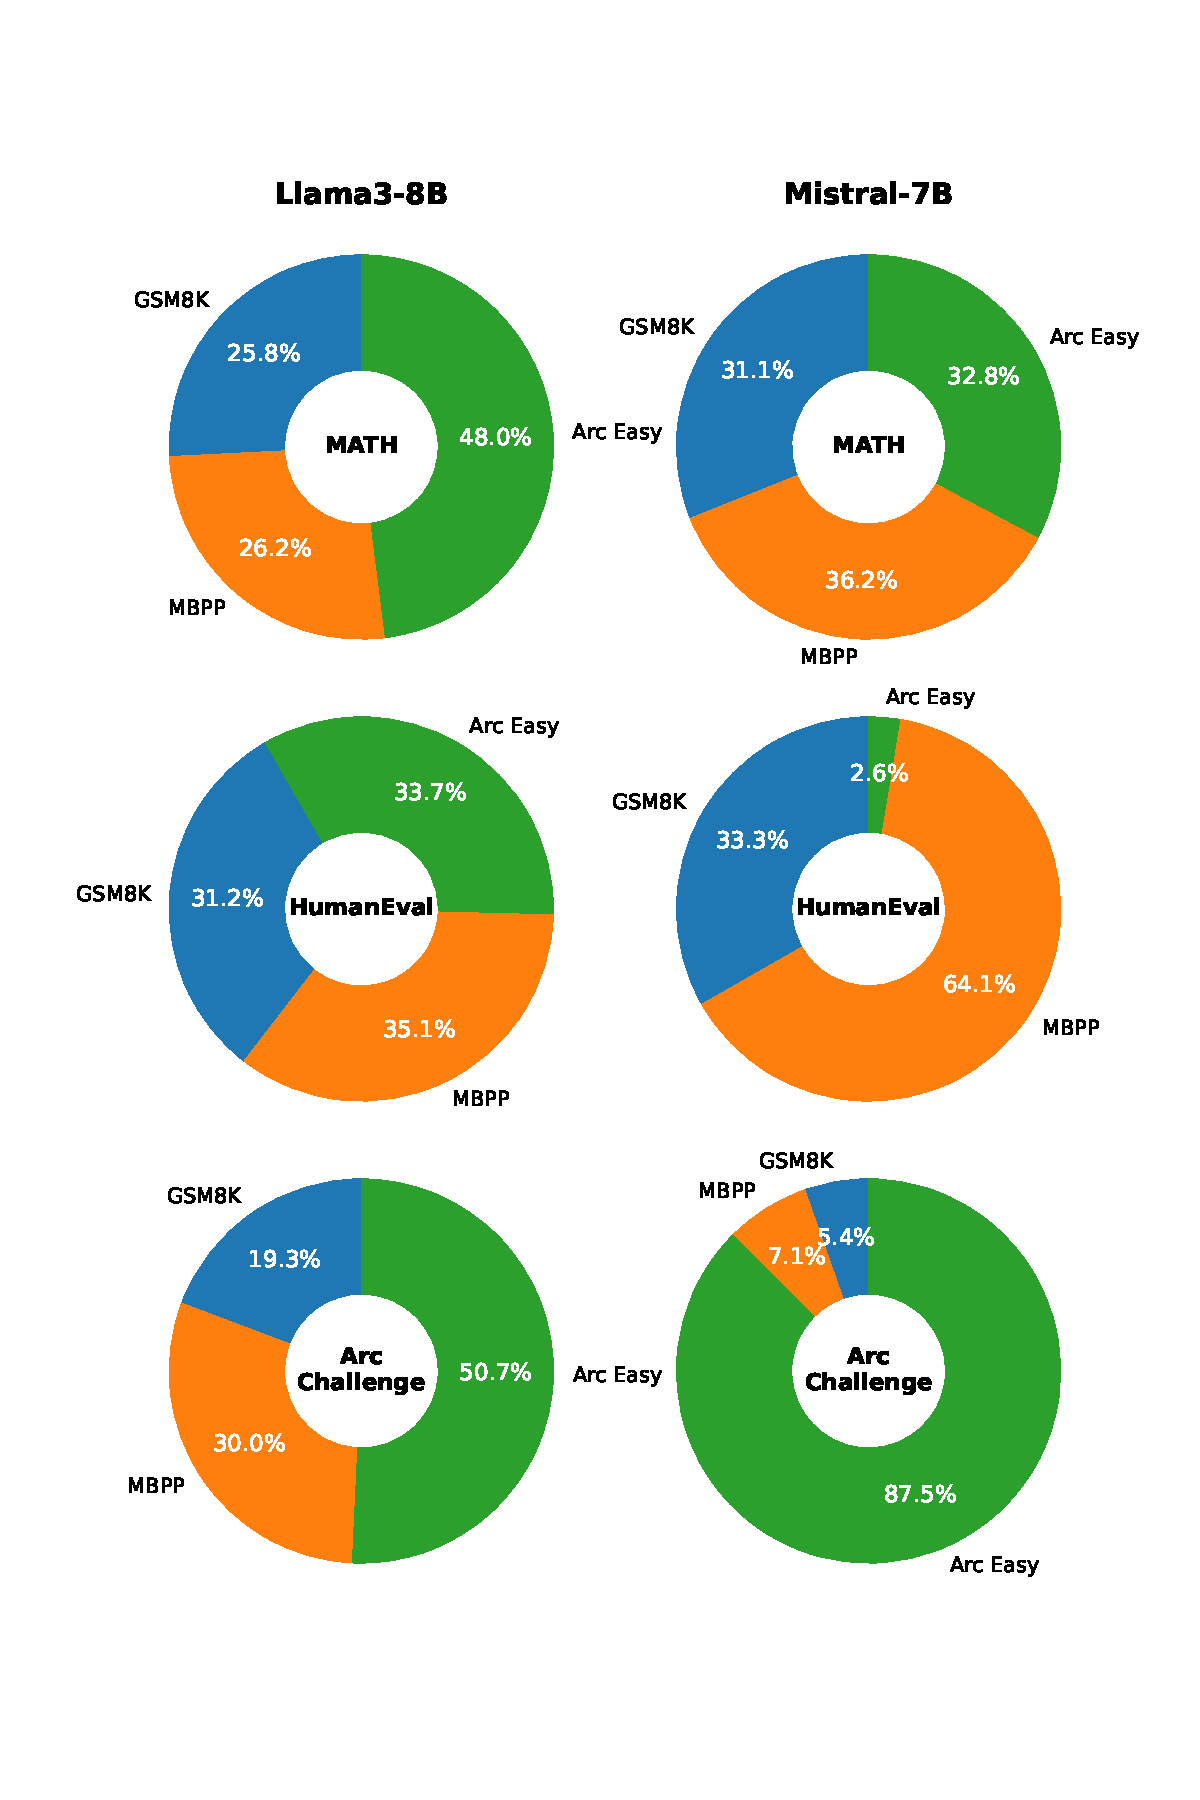
\includegraphics[width=0.32\textwidth]{images/cem_plot_vertical_tb.pdf}
  \end{center}
  \vspace{-10mm}
  \caption{\textbf{$\boldsymbol{\alpha_k}$ learned weights.}}
  \label{fig:cem}
  \vspace{-4mm}
\end{wrapfigure}

This operation leads to notable performance degradation across each task. 
Finally, by performing few-shot adaptation using the \svdacro vectors collected from both models, the performance of \mistral further improves across the board.
We observe that these gains even surpass the best score from adapting \mistral with \textit{all} the \svdacro vectors in the ARC-Challenge task reported in Table~\ref{tab:res:svf_ada_tasks}.  
While these results appear promising, we note that the surprising compatibility discovered through our naive transfer approach is potentially tied to the similarity between the architectures of the two considered LLMs.
To this end, whether similar transfer can be replicated with models of different scales remains an open research question that could open the doors to disentangling and recycling task-specific skills for newer/larger models, with important implications for democratization and sustainability.

\begin{table}[!h]
% \vspace{-4mm}
% \caption{\textbf{Cross-model $z$ vector transfer.}
\caption{\textbf{Cross-model $\boldsymbol{z}$ vector transfer.}
Results from transferring the expert vectors trained on \llama to \mistral with cross model few-shot adaptation.
}
% \vspace{-3.5mm}
\centering
\begin{tabular}{lccc}
\toprule
\textbf{Method} & \textbf{MATH} & \textbf{Humaneval} & \textbf{ARC-Challenge} \\
\textit{SVF training task} & \small{\textit{GSM8K}} & \small{\textit{MBPP-pro}} & \small{\textit{ARC-Easy}} \\
\midrule


\textsc{Mistral-7B-Instruct-v0.3} & \textbf{{\normalsize 13.02 {\footnotesize (\grey{1.00})}}} & {\normalsize 43.29 {\footnotesize (\grey{1.00})}} & {\normalsize 71.76 {\footnotesize (\grey{1.00})}} \\

\midrule

\quad + Llama SVF (ordered $\sigma_i$) & {\normalsize 11.96 {\footnotesize (\red{0.92})}} & {\normalsize 45.12 {\footnotesize (\green{1.04})}} & {\normalsize 72.01 {\footnotesize (\grey{1.00})}} \\
\quad + Llama SVF (shuffled $\sigma_i$) & {\normalsize 10.52 {\footnotesize (\red{0.81})}} & {\normalsize 40.24 {\footnotesize (\red{0.93})}} & {\normalsize 70.82 {\footnotesize (\red{0.99})}} \\
\quad + Few-shot adaptation (cross-model) & {\normalsize 12.65 {\footnotesize (\red{0.97})}} & \textbf{{\normalsize 46.75 {\footnotesize (\green{1.08})}}} & \textbf{{\normalsize 75.64 {\footnotesize (\green{1.05})}}} \\

\bottomrule
\end{tabular}
\label{tab:analysis:cross_model_main}
\vspace{-2mm}
\end{table}
